\documentclass[main.tex,fontsize=8pt,paper=a4,paper=portrait,DIV=calc,]{scrartcl}
% Document
\usepackage[T1]{fontenc}
\usepackage[dvipsnames]{xcolor}
\usepackage[nswissgerman,english]{babel}
\renewcommand{\familydefault}{\sfdefault}

% Format
\usepackage[top=5mm,bottom=1mm,left=5mm,right=5mm]{geometry}
%\setlength{\headheight}{\baselineskip}
%\setlength{\headsep}{0mm}

%\usepackage{scrlayer-scrpage}
%\clearpairofpagestyles
%\chead{{\bfseries\TITLE, \AUTHOR, \pagename~\thepage}}

%\addtokomafont{pagehead}{\upshape}

\usepackage{multicol}
\setlength{\columnsep}{2mm}
\setlength{\columnseprule}{0.1pt}

% Math
\usepackage{amsmath}
\usepackage{amssymb}
\usepackage{amsfonts}

% Code
\usepackage{fancyvrb, etoolbox, listings, xcolor}
%\usemintedstyle{bw}

%\newminted[shell]{bash}{
%fontsize=\footnotesize,
%fontfamily=tt,
%breaklines=true,
%frame=single,
%framerule=0.1pt,
%framesep=2mm,
%tabsize=2
%}
%\newminted{css}{
%breaklines=true,
%tabsize=4,
%autogobble=true,
%escapeinside=||,
%stripall=true,
%stripnl=true,
%}

    \definecolor{lightgray}{rgb}{0.95, 0.95, 0.95}
    \definecolor{darkgray}{rgb}{0.4, 0.4, 0.4}
    \definecolor{purple}{rgb}{0.65, 0.12, 0.82}
    \definecolor{ocherCode}{rgb}{1, 0.5, 0} % #FF7F00 -> rgb(239, 169, 0)
    \definecolor{blueCode}{rgb}{0, 0, 0.93} % #0000EE -> rgb(0, 0, 238)
    \definecolor{greenCode}{rgb}{0, 0.6, 0} % #009900 -> rgb(0, 153, 0)
    \definecolor{teal}{rgb}{0.0, 0.5, 0.5}

\lstdefinestyle{code}{
    identifierstyle=\color{black},
    keywordstyle=\color{blue}\bfseries\small,
    ndkeywordstyle=\color{greenCode}\bfseries\small,
    stringstyle=\color{ocherCode}\ttfamily\small,
    commentstyle=\color{teal}\ttfamily\textit\small,
    basicstyle=\ttfamily\small,
    breakatwhitespace=false,         
    breaklines=true,                 
    captionpos=b,                    
    keepspaces=true,                 
    showspaces=false,                
    showstringspaces=false,
    showtabs=false,                  
    tabsize=2,
    belowskip=-5pt
}



% Images
\usepackage{graphicx}
\newcommand{\pic}{\includegraphics[scale=0.3]}
\graphicspath{{Screenshots/}{../Screenshots}}
\makeatletter
\def\pictext#1#2{%
    \@ifnextchar[{%
    \pictext@iiiii{#1}{#2}%
    }{%
      \pictext@iiiii{#1}{#2}[0.5,0.4,0.3]% Default is 5
    }%
}
\def\pictext@iiiii#1#2[#3,#4,#5]{\begin{minipage}{#3\textwidth}\includegraphics[scale=#4]{#1}\end{minipage}\begin{minipage}{#5\textwidth}#2\end{minipage}}
\def\minipg#1#2{%
    \@ifnextchar[{%
    \minipg@iiii{#1}{#2}%
    }{%
      \minipg@iiii{#1}{#2}[0.3,0.6]% Default is 5
    }%
}
\def\minipg@iiii#1#2[#3,#4]{\vspace{0.8mm}\begin{minipage}{#3\textwidth}#1\end{minipage}\begin{minipage}{#4\textwidth}#2\end{minipage}{\vspace{0.8mm}}}
\makeatother

%\newenvironment{minty}[2]% environment name
%{% begin code
%  \begin{minipage}{#1}
%  \begin{minted}{#2}
%}%
%{% end code
%  \end{minted}
%  \end{minipage}
%  \end{minty}\ignorespacesafterend
%} 

% Smaller Lists
\usepackage{enumitem}
\setlist[itemize,enumerate]{leftmargin=3mm, labelindent=0mm, labelwidth=1mm, labelsep=1mm, nosep}
\setlist[description]{leftmargin=0mm, nosep}
\setlength{\parindent}{0cm}

% Smaller Titles
\usepackage[explicit]{titlesec}

%% Color Boxes
\newcommand{\sectioncolor}[1]{\colorbox{black!60}{\parbox{0.989\linewidth}{\color{white}#1}}}
\newcommand{\subsectioncolor}[1]{\colorbox{black!50}{\parbox{0.989\linewidth}{\color{white}#1}}}
\newcommand{\subsubsectioncolor}[1]{\colorbox{black!40}{\parbox{0.989\linewidth}{\color{white}#1}}}
\newcommand{\paragraphcolor}[1]{\colorbox{black!30}{\parbox{0.989\linewidth}{\color{white}#1}}}
\newcommand{\subparagraphcolor}[1]{\colorbox{black!20}{\parbox{0.989\linewidth}{\color{white}#1}}}

%% Title Format
\titleformat{\section}{\vspace{0.5mm}\bfseries}{}{0mm}{\sectioncolor{\thesection~#1}}[{\vspace{0.5mm}}]
\titleformat{\subsection}{\vspace{0.5mm}\bfseries}{}{0mm}{\subsectioncolor{\thesubsection~#1}}[{\vspace{0.5mm}}]
\titleformat{\subsubsection}{\vspace{0.5mm}\bfseries}{}{0mm}{\subsubsectioncolor{\thesubsubsection~#1}}[{\vspace{0.5mm}}]
\titleformat{\paragraph}{\vspace{0.5mm}\bfseries}{}{0mm}{\paragraphcolor{\theparagraph~#1}}[{\vspace{0.5mm}}]
\titleformat{\subparagraph}{\vspace{0.5mm}\bfseries}{}{0mm}{\subparagraphcolor{\thesubparagraph~#1}}[{\vspace{0.5mm}}]

%% Title Spacing
\titlespacing{\section}{0mm}{0mm}{0mm}
\titlespacing{\subsection}{0mm}{0mm}{0mm}
\titlespacing{\subsubsection}{0mm}{0mm}{0mm}
\titlespacing{\paragraph}{0mm}{0mm}{0mm}
\titlespacing{\subparagraph}{0mm}{0mm}{0mm}

%% format cells
\usepackage[document]{ragged2e}
\usepackage{array, makecell}
\renewcommand{\arraystretch}{2}
\newcommand{\mc}{\makecell[{{m{1\linewidth}}}]}



\lstdefinelanguage{JavaScript}{
  keywords={break, case, catch, continue, debugger, default, delete, do, else, false, finally, for, function, if, in, instanceof, new, null, return, switch, this, throw, true, try, typeof, var, void, while, with},
  morecomment=[l]{//},
  morecomment=[s]{/*}{*/},
  morestring=[b]',
  morestring=[b]",
  ndkeywords={class, export, boolean, throw, implements, import, this},
  keywordstyle=\color{blue}\bfseries,
  ndkeywordstyle=\color{darkgray}\bfseries,
  identifierstyle=\color{black},
  commentstyle=\color{purple}\ttfamily,
  stringstyle=\color{red}\ttfamily,
  sensitive=true
}

%%%%%define html as viable language
\lstset{
    language=JavaScript,
    style=code,
}
%%%%%

\begin{document}
\begin{table}[h!]
\section{Basics}
\begin{tabular}{|m {0.205\linewidth}|m{0.750\linewidth}|}
\hline
ECMAScript & 
Javascript is only an implementation of ECMAScript. So ECMA is the actual standard.\\
\hline 
debug without IDE & 
\begin{lstlisting}
debugger;
\end{lstlisting}
\, \newline
\textcolor{teal}{This simply makes the browser stop at this line if the dev tools are open!}\\
\hline
Facts about javascript & 
\begin{itemize}
  \item \textcolor{teal}{It's dynamic}
  \item \textcolor{teal}{It's dynamically typed! (like python)}
  \item \textcolor{teal}{both functional and object-oriented}
  \item \textcolor{teal}{It fails silently --> "geil"}
  \item \textcolor{teal}{It's deployed as source code, so everything is at least source available}
  \item \textcolor{teal}{It's part of the web platform}
\end{itemize}
\\
\hline
\textbf{Primitives vs Objects} & 
\large\textcolor{red}{Primitives}
\normalsize
\begin{itemize}
  \item \textcolor{teal}{string, number, boolean, undefined}
  \item \textcolor{teal}{compared by value}
  \item \textcolor{teal}{always immutable}
\end{itemize}
\, \newline
\large\textcolor{red}{Objects}
\normalsize
\begin{itemize}
  \item \textcolor{teal}{Arrays, Regular Expressions, Functions}
  \item \textcolor{teal}{compared by Reference}
  \item \textcolor{teal}{Mutable by default}
  \vspace{-3mm}
\end{itemize}
\\
\hline
Types & 
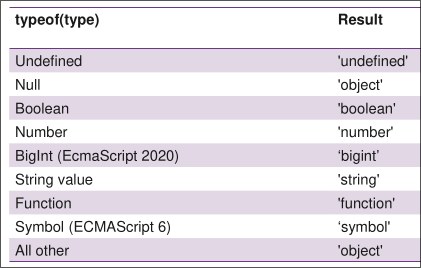
\includegraphics[scale=0.45]{2022-10-11-10:33:44.png}\\
\hline
Boolean Checks & 
\textcolor{red}{Every value can be converted to a boolean}\newline
\begin{itemize}
  \item !!(null) => false
  \item Boolean( null ) => false
\end{itemize}
\, \newline
\begin{itemize}
  \item \textcolor{teal}{Logical Operators \&\& ||}
  \item \textcolor{teal}{Not !}
  \item \textcolor{teal}{Equality Checks === !== > >= < <=} true or false
  \item \textcolor{teal}{Value Equality Check == !=} true false or NaN -> cast to number
  \vspace{-3mm}
\end{itemize}
\, \newline
\minipg{
True Values:\newline
\begin{itemize}
  \item false
  \item 0 
  \item "" 
  \item null 
  \item undefined 
  \item NaN
\end{itemize}
}
{True Values:
\begin{itemize}
  \item "0" \textcolor{teal}{any string that has something in it is considered true}
  \item "false"
  \item \char`\[ \char`\]
  \item \char`\{ \char`\}
\end{itemize}}\\
\hline 
NaN &
\vspace{2mm}
\begin{itemize}
  \item \textcolor{red}{is an error value} 
  \item 0 / 0 = NaN
  \item is of type number
  \item NaN == NaN is false \textcolor{teal}{// use isNan\char`\( \char`\) instead}
  \vspace{-3mm}
\end{itemize}\\
\hline
Infinity & 
Infinity is a number in js, can be used to represent the mathematical infinity.\newline
Will also be used if the number is too big!\\
\hline
Numbers & 
\textcolor{red}{Every value can be casted to a number!}\newline
\begin{itemize}
  \item +(true) = 1
  \item Number(true) = 1
  \item Number(null) = 0
  \item Number("abc") = NaN \textcolor{teal}{remember NaN is of type number!}
  \item one exception -> symbol, this is not a number
  \vspace{-3mm}
\end{itemize}\\
\hline
String & 
\textcolor{teal}{Can be represented with either "" or ''}\newline
\textcolor{teal}{Escape character is \textbackslash}\newline
\minipg{
Typical Methods:\newline
\begin{itemize}
  \item length
  \item slice
  \item trim\char`\( \char`\)
  \item includes\char`\( \char`\)
  \item indexOf\char`\( \char`\)
\end{itemize}
}
{
  Special Operations:
  \textcolor{red}{Number + String = String}\newline
  \textcolor{red}{String + Number = String}\newline
}\\
\hline
\end{tabular}
\end{table}
\pagebreak
\begin{table}[ht!]
\begin{tabular}{|m{0.2\linewidth}|m{0.755\linewidth}|}
\hline
null / undefined & 
\textcolor{teal}{Undefined means nothing, not yet defined}\newline
\textcolor{teal}{null is a value, the null value}\newline
\textcolor{red}{IMPORTANT: null == undefined = true !!}\newline
Example with null and undefined:\newline
\begin{lstlisting}
import * as userList
from './user.mjs';
console.log( userList.get(0) );
console.log( userList.update(0, {birthday: "19.05.1986"}) );
console.log( userList.update(0, {name : undefined, birthday: "19.05.1986"}) );
console.log( userList.update(0, {name : null, birthday: "19.05.1986"}) );
{ name: 'Michael', birthday: '19.05.1985' }
{ name: 'Michael', birthday: '19.05.1986' }
{ name: 'Michael', birthday: '19.05.1986' }
{ name: null, birthday: '19.05.1986' }
\end{lstlisting}
\\
\hline
Array & 
\begin{lstlisting}
const arr = [ 'a', 'b', 'c' ];
arr[0] = 'x';
arr.push("d");
console.log(arr); // [ 'x', 'b', 'c', 'd' ]
console.log(arr.length); // 4
\end{lstlisting}
\, \newline
This is the list for everything.\newline
\begin{itemize}
  \item \textcolor{teal}{no fix length}
  \item \textcolor{teal}{index starts at 0}
  \vspace{-3mm}
\end{itemize}
\, \newline
\, \newline
\textcolor{orange}{\textbf{To check if something is an array you can compare constructors!}}\newline
\begin{lstlisting}
function isArray(arr) {
  if(arr.constructor === Array) {
    return true;
  }
  return false;
}
\end{lstlisting}
\, \newline
\textcolor{teal}{arr.forEach}\newline
\begin{lstlisting}
let sum = 0;
arr.forEach(num => { sum += num });
\end{lstlisting}
\, \newline
\textcolor{teal}{arr.reduce}\newline
\begin{lstlisting}
const sum = arr.reduce((total, n) => total + n, 0);
\end{lstlisting}
\\
\hline
For Loops & 
\textcolor{teal}{classic:}\newline
\begin{lstlisting}
for(let i=0; i<arr.length; ++i) {
  console.log("for",arr[i]);
} // like regular loop just with let
\end{lstlisting}
\, \newline
\textcolor{teal}{For-In:}\newline
\begin{lstlisting}
for(const x in arr) {
  console.log("for in", x + ":" + arr[x]);
} // !! this returns the index string not the element !!
\end{lstlisting}
\, \newline
\textcolor{teal}{For-Of:}\newline
\begin{lstlisting}
for(const y of arr) {
  console.log("for of", y);
} // like for(auto e : arr)
\end{lstlisting}
\\
\hline
Object & 
\textcolor{teal}{An object is a collection of properties}\newline
These values are stored in a \textbf{key | value} -> \textbf{HashSet}.\newline
\begin{lstlisting}
cosnt person = {
  name: "spass"
  func: function() {
    return this.name;
  }
};
person.name = "Bob";
person.func();
\end{lstlisting}\\
\hline
Mutability of Objects & 
\textcolor{teal}{You can overwrite functions inside of these objects!}\newline
\begin{lstlisting}
person.func = function() {
  console.log("this does something else now !");
}
\end{lstlisting}\\
\hline
Functions &
\textcolor{teal}{As expected, functions are first class citizens, aka they can be variables!}\newline
\begin{lstlisting}
func = printSomething() {
  console.log("ping pang");
}
func();
\end{lstlisting}
\, \newline
Or You can use something like lambdas:\newline
\begin{lstlisting}
const func = (value) => {
  console.log(value);
}
func(5); // prints 5
\end{lstlisting}\\
\hline
\end{tabular}
\end{table}
\pagebreak
\begin{table}[ht!]
\begin{tabular}{|m{0.2\linewidth}|m{0.755\linewidth}|}
\hline
Parameters & 
\large\textcolor{red}{in javascript you can call functions with too many parameters, they will simply be stored in a buffer!!}\newline
\normalsize
\begin{lstlisting}
function foo(name, ...params){
console.log(1,name);
console.log(2,params.join(";"));
}
foo("Michael", "Gfeller", "OST", "IFS");
// prints "Michael" and "Gfeller;OST;IFS"
\end{lstlisting}\\
\hline
& \large \textcolor{teal}{Properties of functions}\newline
\normalsize
\begin{lstlisting}
const fn1 = function(){ return "Michael" };
console.log(fn1.name);
// ""

const fn2 = function name(){ return "Michael" };
console.log(fn2.name);
// "name"
console.log(fn2.length); // 0

const fn3 = function name(name){ return name };
console.log(fn3.length); // 1
\end{lstlisting}
\, \newline
\large \textcolor{red}{!!! Javascript doesn't have function overloading !!!}\newline
\normalsize The solution is to use if statements inside those functions with \textbf{typeof}\newline
\begin{lstlisting}
jQuery.fn.init = function( selector, context ) {
//...
if ( !selector ) {
return this;
}
// Handle HTML strings
if ( typeof selector === "string" ) {
//...
} else if ( selector.nodeType ) {
//...
} else if ( jQuery.isFunction( selector ) ) {
//...
}
//...
return jQuery.makeArray( selector, this );
};
\end{lstlisting}\\
\hline
\end{tabular}
\end{table}
\pagebreak
\begin{table}[ht!]
\section{DOM Document Object Model}
\begin{tabular}{|m{0.2\linewidth}|m{0.755\linewidth}|}
\hline
window & 
\textcolor{orange}{This simply provides global objects such as \textbf{console, document and HTMLDocument}}\newline
\textcolor{teal}{All global variables reside here.}\\
\hline
Selection &
\textcolor{orange}{There are different ways of selecting an element or node:}\newline
\begin{itemize}
  \item \textcolor{teal}{document.querySelector('name')} // select by CSS syntax -> also allows css selectors!
  \item \textcolor{teal}{document.querySelectorAll('.nav')} // select All by CSS syntax -> also allows css selectors!
  \item \textcolor{teal}{document.getElementById('list-container')} // select by id
  \item \textcolor{teal}{document.getElementByTagName('li')} // select by Tag name
  \item \textcolor{teal}{document.getElementsByClassName('nav-item')} // select by class name
\end{itemize}
\, \newline
\textcolor{orange}{Just use the querySelector -> it allows more ways to select it! \newline
However theoretically the html selectors are faster!}\\
\hline
DOM-Manipulation by create & 
\textcolor{orange}{We can also create new elements with js the same way we select elements}\newline
\begin{lstlisting}
const newEl = document.createElement('div');
newEl.appendChild(document.createTextNode('Hello'));
document.querySelector("#container").appendChild(newEl);
\end{lstlisting}
\, \newline
\pic{2022-10-18-11:26:10.png} \pic{2022-10-18-11:26:36.png}\newline
\textcolor{orange}{this is faster with small changes, DOM references stay the same, event handlers stay alive}\\
\hline
DOM-Manipulation by innerHTML & 
\begin{lstlisting}
const c = document.querySelector('#container');
c.innerHTML = '<div>Ping pang!</div>';
\end{lstlisting}
\, \newline
\textcolor{orange}{this is likely faster and more readable}\\
\hline 
DocumentFragment & 
\textcolor{orange}{This creates a temporary fragment that will be deleted when attaching this to a parent node.}\newline
\begin{lstlisting}
document.createDocumentFragment();
\end{lstlisting}
\, \newline
\pic{2022-10-18-11:31:01.png}\\
\hline
EventListener & 
\textcolor{orange}{An event listener is used to bind a function to something like a button\newline
For example a darkmode button is mapped to the useDarkMode function}\newline
\begin{lstlisting}
document.querySelector('button')
.addEventListener('click' // action to map , useDarkMode // function to map,[options] // once, capture etc)
\end{lstlisting}
\\
\hline
remove Eventlistener \newline and dispatchEvent & 
You can of course also remove an eventlistener, or execute an event per js call:\newline
\begin{lstlisting}
document.querySelector('button').removeEventListener('click', useDarkMode);
// remove eventlistener

document.querySelector('button').dispatchEvent('click');
// dispatch the click event
\end{lstlisting}\\
\hline
NodeStructure & 
\textcolor{orange}{HTML is built like a tree with different nodes and leafs.}\newline
\textcolor{teal}{Important is that there are different types of nodes that html uses}\newline
\begin{itemize}
  \item \textcolor{orange}{ElementNode} head,body,li,title etc
  \item \textcolor{orange}{AttributeNode} href, charset, src etc
  \item \textcolor{orange}{TextNode} some text to display
  \item \textcolor{orange}{Comments} <!-- kekw -->
  \vspace{-3mm}
\end{itemize}
\, \newline
\pic{2022-10-18-10:35:52.png}
\\
\hline
\end{tabular}
\end{table}
\pagebreak
\begin{table}[ht!]
\begin{tabular}{|m{0.2\linewidth}|m{0.755\linewidth}|}
\hline
\textbf{async and defer} & 
\textcolor{orange}{\textbf{async:} Async means that the script will be loaded and executed immediately.\newline
This means that there \textbf{is no guarantee for order} and the script will be \textbf{executed before the document has loaded}.}\newline
\textcolor{blue}{\textbf{defer:} This is the opposite to async, it will \textbf{gurarantee order}, \newline
and the document will \textbf{be loaded before the script executes}.}\newline
\pic{2022-10-18-10:45:27.png}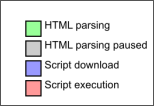
\includegraphics[scale=0.4]{2022-10-18-10:46:00.png}\newline
\textcolor{orange}{\textbf{If you want to check whether or not the document is ready, \newline
then you can do this with: }}\textcolor{red}{\textbf{\emph{document.readyState}}}
\\
\hline
TextContent and innerText & 
\textcolor{orange}{HTMLElement.innerText provides the rendered text with css applied}\newline
\textcolor{blue}{HTMLElement.textContent provides the complete raw text with no css applied}\\
\hline 
className and classList & 
\begin{lstlisting}
<script>
console.log(
document.querySelector("#el").className);
// box alert important

console.log(document.querySelector("#el")
.classList);
// DOMTokenList(3) ["box", "alert", "important"]
</script>
\end{lstlisting}\\
\hline
\end{tabular}
\subsection{Event Handling}
\begin{tabular}{|m{0.2\linewidth}|m{0.755\linewidth}|}
\hline
EventListener with options & 
\begin{lstlisting}
target.addEventListener(type, listener[, options]);
\end{lstlisting}
\, \newline
options:\newline
\begin{itemize}
  \item capture
  \item once
  \item 
  \vspace{-3mm}
\end{itemize}\\
\hline
Event Listener vs inline & 
\begin{lstlisting}
<HTMLElement>.addEventListener()
document.querySelector("#1").addEventListener("click", () => alert('1'));
// multiple listeners possible!

<HTMLElement>.on... = eventHandler
document.querySelector("#2").onclick = () => alert('2');
// only 1 listener possible
// will overwrite previous onclick assignments

<button onclick="alert('3')">3</button>
// provides the least amount of flexibility, not recommended
\end{lstlisting}\\
\hline
Event Phases & \minipg{
\textcolor{orange}{Events go through 3 phases:}\newline
\begin{enumerate}
  \item \textcolor{teal}{Capture-Phase}\newline
    Event travels from root to leaf\newline
    Every Element can react here
  \item \textcolor{teal}{Target-Phase}\newline
    Event will be destroyed on target
  \item \textcolor{teal}{Bubble-Phase}\newline/
    Event travels from leaf to root\newline
    Each element can react
\end{enumerate}
\, \newline
\textcolor{orange}{Event bubbling and capture is used to dynamically change lists, etc.}
}
{\pic{2022-10-18-12:15:49.png}}[0.3,0.4]\\ 
\hline
\end{tabular}
\end{table}
\pagebreak
\begin{table}[!ht]
\subsection{Node}
\begin{tabular}{|m{0.2\linewidth}|m{0.755\linewidth}|}
\hline
Important Properties and functions & 
\textcolor{orange}{\textbf{Properties}}
\begin{itemize}
  \item \textcolor{teal}{children} only nodes of type HTMLelement 
  \item \textcolor{teal}{childNodes} 
  \item \textcolor{teal}{firstChild} first node child
  \item \textcolor{teal}{firstElementChild} first element child
  \item \textcolor{teal}{nextSibling} next node sibling
  \item \textcolor{teal}{nextElementSibling} next element 
  \item \textcolor{teal}{parentElement} 
\end{itemize}
\, \newline
\textcolor{orange}{Functions}\newline
\begin{itemize}
  \item \textcolor{teal}{appendChild()}
  \item \textcolor{teal}{removeChild()}
  \vspace{-3mm}
\end{itemize}\\
\hline
\end{tabular}
\subsection{Element}
\begin{tabular}{|m{0.2\linewidth}|m{0.755\linewidth}|}
\hline
Important Properties and functions & 
\textcolor{orange}{\textbf{Properties}}
\begin{itemize}
  \item \textcolor{teal}{id} 
  \item \textcolor{teal}{className} 
  \item \textcolor{teal}{classList} 
  \item \textcolor{teal}{innerHTMl}
\end{itemize}
\, \newline
\textcolor{orange}{Functions}\newline
\begin{itemize}
  \item \textcolor{teal}{getAttribute()}
  \item \textcolor{teal}{setAttribute()}
  \item \textcolor{teal}{toggleAttribute()}
  \item \textcolor{teal}{closest()}
  \vspace{-3mm}
\end{itemize}\\
\hline
Element ParentNode & 
\textcolor{orange}{Element also implements Parentnode:}\newline
Properties:\newline
\begin{itemize}
  \item \textcolor{teal}{children}
  \item \textcolor{teal}{firstElementChild}
  \item \textcolor{teal}{lastElementChild}
\end{itemize}
\, \newline
Functions:\newline
\begin{itemize}
  \item \textcolor{teal}{append()} 
  \item \textcolor{teal}{remove()}
  \vspace{-3mm}
\end{itemize}\\
\hline
\end{tabular}
\subsection{HTMLElement}
\begin{tabular}{|m{0.2\linewidth}|m{0.755\linewidth}|}
\hline
Important Properties and functions & 
\textcolor{orange}{\textbf{Properties}}
\begin{itemize}
  \item \textcolor{teal}{dataset} 
  \item \textcolor{teal}{style} 
  \item \textcolor{teal}{hidden}
\end{itemize}
\, \newline
\textcolor{orange}{Functions}\newline
\begin{itemize}
  \item \textcolor{teal}{createCaption()}
  \item \textcolor{teal}{createTFoot()}
  \item \textcolor{teal}{createTHead()}
  \vspace{-3mm}
\end{itemize}\\
\hline
\end{tabular}
\subsection{Event-Object}
\begin{tabular}{|m{0.2\linewidth}|m{0.755\linewidth}|}
\hline
Important Properties and functions & 
\textcolor{orange}{\textbf{Properties}}
\begin{itemize}
  \item \textcolor{teal}{target} // element of event origin 
  \item \textcolor{teal}{currentTarget} // element that has listener for this event
\end{itemize}
\, \newline
\textcolor{orange}{Functions}\newline
\begin{itemize}
  \item \textcolor{teal}{preventDefault()} // prevents default actions like automatic form submit
  \item \textcolor{teal}{stopPropagation()} // stops capturing and bubbling
\end{itemize}
\, \newline
\textcolor{orange}{Specific Event types}\newline
\begin{itemize}
  \item \textcolor{teal}{MouseEvent}
  \item \textcolor{teal}{WheelEvent}
  \item \textcolor{teal}{InputEvent}
  \item \textcolor{teal}{KeyboardEvent}
  \vspace{-3mm}
\end{itemize}\\
\hline
Keyboard Event & 
\begin{lstlisting}
<body>
<input>
<script>
document.querySelector("input").addEventListener("keydown", (event) => {
console.log(event.key);
})
</script>
\end{lstlisting}
\minipg{
\begin{itemize}
  \item change: what changed?
  \item keydown: which key has been pressed?
  \item ctrlKey: was the control pressed during keydown?
  \vspace{-3mm}
\end{itemize}
}
{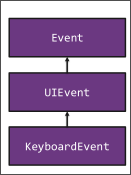
\includegraphics[scale=0.5]{2022-10-18-12:33:39.png}}[0.35,0.4]\\
\hline
\end{tabular}
\end{table}
\pagebreak
\begin{table}[ht!]
\section{Scopes}
\begin{tabular}{|m{0.2\linewidth}|m{0.755\linewidth}|}
\hline
Var vs let & 
\textcolor{orange}{Usually we declare variables using the let keyword, however, the old var keyword still has one technicality that the let keyword doesn't have. Namely the var keyword will always be available for the parent scope:}\newline
\begin{lstlisting}
{ // empty explicit scope to show difference
  function some_func() {
    let num1 = 5;
    var num2 = 6;
    console.log(num1); // ok -> 5
    console.log(num2); // ok -> 6
  }
    console.log(num1); // -> undefined!
    console.log(num1); // ok -> 6
}
\end{lstlisting}\\
\hline
Scope per file in NodeJs &
\textcolor{orange}{NodeJs creates an additional scope per file, this means that you essentially can only explicitly declare a truly global variable with var.}\newline
\textcolor{red}{However, the browser does \textbf{NOT} have this feature!}\\
\hline
Closure & 
\textcolor{orange}{This is just the concept of boxing a something in something and then accessing the scope from the inner "something". Usually done with functions:}\newline
\begin{lstlisting}
function something1() {
  let num = 5;
  function something2() {
    console.log(num); // obviously works
  }
}
\end{lstlisting}\\
\hline
global Scope & 
\textcolor{orange}{If you access a global variable, it is probably better to use the \textbf{global.variable} naming scheme. The reason for this is obviously the fact that you don't use the variable of another scope by accident.}\\
\hline
This in scopes & 
\textcolor{orange}{if we do not have an object, then the \textbf{the global scope will be this!}\newline
This means that you can do things like this:}\newline
\begin{lstlisting}
function printName() {
  console.log(this.name);
}

const name = "ping"

const logEntry = {
  name: "pang"
};

logEntry.printName = printName;
logEntry.printName(); // will print "pang"
printName(); // will print "ping" -> empty object will always invoke the global object!!
\end{lstlisting}\\
\hline
Functions with new (old js) & 
\textcolor{orange}{Before proper OOP was introduced, this was the way you wrote OOP in js:}\newline
\begin{lstlisting}
// given the code from above, we create another printName instance with new
// this will create an empty object that will be the "instance" to call the method on
new printName();

// This is what happens under the hood when you call new printName()!
// function newPrintName() {
//   var self = {}
//   console.log(self.name);
//   return self;
// }
\end{lstlisting}\\
\hline
This as a parameter & 
\textcolor{orange}{You can also pass the this keyword as a parameter!}\newline
\begin{lstlisting}
logEntry.printName({name: "pingpang"});
// this will print "pingpang" instead of the logEntry name "pang" !!
\end{lstlisting}\\
\hline
Bind & 
\textcolor{orange}{You can also "bind" a certain "this" to one function in particular, this means that all other function other than the one you bound, will be used with the regular "this"!!}\newline
\begin{lstlisting}
const bindPrintName = logEntry.printName({ name: "burrmiu" });
bindPrintName(); // this will ALWAYS print "burrmiu"
// at least until you override it!
bindPrintName({name: "pangPing!"}); // !!!! this will still print "burrmiu" !!!!
\end{lstlisting}\\
\hline
\end{tabular}
\section{strict}
\begin{tabular}{|m{0.2\linewidth}|m{0.755\linewidth}|}
\hline
Basic & 
\textcolor{orange}{This disables certain JS features that might be unwanted in this particular usecase. \newline
It can be enabled per Scope or per file}\newline
\textcolor{purple}{Usually this simply makes JS throw an exception when you would expect it from other functions,for example when using a method with a "this" but used on nothing -> exception instead of using global scope.}\\
\hline
Usage & 
\begin{lstlisting}
function someFunc() {
  'use strict'; // this enables the strict mode for this particular scope or file
  // for compatability, should a browser use old js without this feature, then the strict will simply be ignored
}
\end{lstlisting}\\
\hline
General & 
\textcolor{orange}{All new features in JS are in strict mode, this essentially forces us to use it, and it is generally good practice to simply use the strict mode!}\\
\hline
\end{tabular}
\end{table}
\pagebreak
\begin{table}[ht!]
\section{Lambda}
\begin{tabular}{|m{0.2\linewidth}|m{0.755\linewidth}|}
\hline
Notation & 
\begin{lstlisting}
let x = (parameter) => {
  // Do something
  console.log(parameter);
};
x(5); // will print 5!
\end{lstlisting}\\
\hline
This in Lambda &
\textcolor{orange}{In Lambdas the this is always based on the parent scope.\newline
For example within a function or a class the this will be based on that function or class:}\newline
\begin{lstlisting}
function Point(x, y){
this.x = x;
this.y = y;
this.area = () => this.x + this.y;
}

var areaFn = new Point(10,50).area;
console.log(areaFn());

// explicit version!
// function Point(x, y) {
//   var _this = this; // here the _this is mapped to this!
//   this.x = x;
//   this.y = y;
//   this.area = function () {
//     return _this.x + _this.y;
//   };
// }
\end{lstlisting}\\
\hline
\end{tabular}
\section{Objects and Classes}
\begin{tabular}{|m{0.2\linewidth}|m{0.755\linewidth}|}
\hline
Objects are Hashtables! & 
\textcolor{orange}{Every object is a hashtable, this means that we have different means to access it's values. \newline
The same thing therefore applies to arrays as well as long as there is a name for it:}\newline
\begin{lstlisting}
const items = {name: "pingpang"};

console.log(items.name);
console.log(items["name"]);
// these are both the same!
\end{lstlisting}
\, \newline
\textcolor{purple}{Since js does not have static types, you can also add something like name: "ping" to an array and access it the same way you access any other object, however this is \textbf{not recommended!}}\\
\hline
Classes &
\vspace{2mm}
\begin{itemize}
\item \textcolor{purple}{\#: This is the prefix for private variables}
\item \textcolor{purple}{super: Superclass call}
\item \textcolor{purple}{instanceof: this checks whether or not,\newline
  an instance is an object of class xyz\newline
Note, subclasses are also instanceof parentclass!}
\vspace{-3mm}
\end{itemize}
\begin{lstlisting}
class Clock {
  #timer // the # makes it private!
  currentTime
  constructor(param) {
    super();
  }
  start() {
    this.#timer = setTimeout(() => { 
      this.currentTime = new Date();
    }, 1000);
  }
  get time() {
    return this.currentTime
  }
  set time(newTime) {
    this.currentTime = newTime
  }
}

const clock = new Clock(); // instance
\end{lstlisting}\\
\hline
Classes before JS6 & 
\textcolor{orange}{The prototype keyword was used to use OOP before JS6, this is still used under the hood, but do not use this anymore unless you have performance issues.}\\
\hline
This Context with Lambda Callbacks &
\textcolor{red}{This code below does not work, the reason for this is that when we pass person.wackUP, we lose the this context, as we only pass the function itself!}\newline
\begin{lstlisting}
class Person {
  constructor(name) {
    this.name = name;
  }

  wackUp() {
    console.log(`${this.name} is awake!`)
  }
}
class Alarm {
  registerAlarm(callback) {
    setTimeout(() => {
      callback()
    }, 1000);
  }
}
const person = new Person("Michael");
const alarm = new Alarm();
alarm.registerAlarm(person.wackUp);
\end{lstlisting}
\\
\hline
\end{tabular}
\end{table}
\pagebreak
\begin{table}[ht!]
\begin{tabular}{|m{0.2\linewidth}|m{0.755\linewidth}|}
\hline
&
\textcolor{red}{In order to preserve the context, we can pass the function as a lambda:}\newline
\begin{lstlisting}
alarm.registerAlarm(() => person.wackUP() );
\end{lstlisting} 
\, \newline
\textcolor{red}{The same can be done in the class itself!!}\newline
\begin{lstlisting}
wackUp = () => {
  console.log(`${this.name} is awake!`)
}
\end{lstlisting}\\
\hline
\end{tabular}
\section{Modules}
\begin{tabular}{|m{0.2\linewidth}|m{0.755\linewidth}|}
\hline
UseCase & 
\textcolor{orange}{The use case is as expected the prevention of namespace issues.\newline
For example every script in the browser is in the global scope, this means that if the index.js and the home.js both have a function called hello(), then they will overwrite each others definition!!}\newline
\textcolor{purple}{The other usecase is \textbf{dependency solving} and \textbf{code departmentalization}.}\newline
\textcolor{teal}{In Node.js the file need to end with .mjs in order to use modules, in the browser the ending .js is fine.}\newline
\textcolor{teal}{Modules are \textbf{ALWAYS STRICT!}}\\
\hline
Definition & 
\textcolor{purple}{\textbf{Modules simply export or import values and functionality to or from other modules!}}\\
\hline
Module Usage & 
\textcolor{red}{\textbf{In order to use a module, the file itself needs to be a module!}}\newline
\begin{lstlisting}
<script src="index.js" type="module"></script>
\end{lstlisting}
\, \newline
\textcolor{orange}{The usage is done with the import keyword:}\newline
\begin{lstlisting}
import {register as alarmClock} from './libs/alarm-clock.js'
import {register as newsFeed} from './libs/news-feed.js'
import * from './pingpang.js' // import every export from this file 
import defaultExport from './something.js' // default export explained below
\end{lstlisting}\\
\hline
Export& 
\textcolor{purple}{There are 2 types of exports, \textbf{named} and \textbf{unnamed}.}\newline
\, \newline
\textcolor{orange}{\textbf{Named Export}: In order to export a function or value, you need to use the export keyword before that function/value:}\newline
\begin{lstlisting}
export someFunc() {
  console.log("pingpang");
}
\end{lstlisting}
\, \newline
\textcolor{orange}{\textbf{defaultExport}: Here we define an export at the end of the file:}\newline
\begin{lstlisting}
export default {name: "pangping"};

// in the import file
console.log(defaultExport.name);
\end{lstlisting}
\\
\hline
\end{tabular}
\section{Advanced JS Features}
\begin{tabular}{|m{0.2\linewidth}|m{0.755\linewidth}|}
\hline
Spread & 
\textcolor{orange}{Spread is a feature that allows fast and easy concatenation of arrays just like in haskell:}\newline
\begin{lstlisting}
const listA = [1,2,3,4,5];
const listB = [10,11,12,13,14];
const listC = [...listA, ...listB];

// this can also be done with other objects

const objA = {name: "pingpang"};
const objB = {name: "pangping"};
const objC = {...objA,...objB}; // this copies the values of objA and objB into objC
const objD = {objA,objB}; // this however copies the full object into it

console.log(objC); // {name: "pingpang", name: "pangping"}
console.log(objD); // {{name: "pingpang"}, {name: "pangping"}}
// note the extra curly braces on the objD -> deep copy!
\end{lstlisting}\\
\hline
Spread Operator as parameter & 
\textcolor{orange}{You can also enter an array as a parameter:}\newline
\begin{lstlisting}
function something(a,b,c) {
  return a + b + c;
}
const arr = [1,2,3,4,5,6,7,8,9];
something(...arr); // this works -> a=1,b=2,c=3,a2=4,b2=5....
\end{lstlisting}\\
\hline
Destructuring & 
\textcolor{orange}{You can create variables directly from an array or object:}\newline
\begin{lstlisting}
const [a, b] = [10,20]; // a = 10, b = 20 
const {c, d} = {name: "pang", price: 50};

function something({message}) {
  console.log(message);
}
something({message:"pangping"}) // prints "pangping"!

function printWithDefaults({message = "message"} = {}) { // object destructuring
console.log(message);
}
printWithDefaults({code: "error_1"}) // error_1
printWithDefaults() // message
\end{lstlisting}\\
\hline
Nullish Operator & 
\textcolor{orange}{In case you want to check if for example a number exists, even a 0, you can use the nullish operator.\newline
This will simply use the value in case it exists, or the default value that you have specified if it is undefined or null.}\newline
\begin{lstlisting}
console.log(0 ?? 42); // will print 0 
console.log(undefined ?? 42); // will print 42
\end{lstlisting}\\
\hline
\end{tabular}
\end{table}
\pagebreak
\begin{table}[ht!]
\begin{tabular}{|m{0.2\linewidth}|m{0.755\linewidth}|}
\hline
Optional chaining & 
\textcolor{orange}{In JS you might always encounter values that are undefined, this often leads to issues where you call a function with undefined values, or even worse the entire function is undefined.\newline
We can counteract this with the Optional Operator:}\newline
\begin{lstlisting}
const item = {
  name: "pangping",
  price: 10, 
  fun: {
    word: "no"
  }
};
console.log(item.fun?.word); // this will print "no" IF the fun object exists!
// otherwise we simply do not execute this code, no exception will be thrown.
\end{lstlisting}\\
\hline
\end{tabular}
\section{Clean Code}
\begin{tabular}{|m{0.2\linewidth}|m{0.755\linewidth}|}
\hline
Naming & 
\textcolor{orange}{Names of variables, function etc should be \textbf{short, intuitive and explicit}.}\newline
\textcolor{teal}{Also the names should be \textbf{spellable} and consisting of \textbf{kown words}, something that you can't say is useless in coop programming.}\newline
\textcolor{purple}{Avoid repeating yourself, if the app is about webtrc, you don't need to specify this every time!}\\
\hline
Naming schemes & 
\textcolor{orange}{There are different schemes for different types of variables that you use.}\newline
\begin{itemize}
\item \textcolor{purple}{regular variables and functions >> camelCase}
\item \textcolor{purple}{constants >> ALL\_CAPS}
\item \textcolor{purple}{boolean values >> isValue}
\item \textcolor{purple}{arrays >> pluralNaming}
\vspace{-2mm}
\end{itemize}\\ 
\hline

\hline

\hline

\hline

\hline

\hline

\hline
\end{tabular}
\end{table}
\pagebreak
\begin{table}[ht!]
\section{PolyFill and BabelJS}
\begin{tabular}{|m{0.2\linewidth}|m{0.755\linewidth}|}
\hline
BabelJS & 
\textcolor{orange}{BabelJS converts new and modern JS code into old style JS, this is used for compatibility with older browsers that do not support the new features.}\\
\hline
PolyFill &
\textcolor{orange}{BabelJS has certain limitations that PolyFill tries to essentially "fill in". This further increases the compatibility with older browsers, however, this still is limited to a certain extend.\newline
For example due to the translating, the performance will be much worse, and considering we are already using an older browser, this can quickly get out of hand.}\\
\hline

\hline

\hline

\hline

\hline

\hline

\hline

\hline

\hline
\end{tabular}
\end{table}
\end{document}
